\chapter{Introdução}
Desenhos de superfícies costumam ser feitos a partir de um ponto de vista do
espaço ambiente 3D ou 2D, como em MatLab, Mathematica e Geogebra.
Uma curva ou superfície é definida numa linguagem e então é renderizada.
Uma forma muito comum de renderização é a discretização da curva ou superfície,
formando segmentos no caso de uma curva, ou triângulos para superfícies.
O usuário então é um observador externo à superfície, posicionado no espaço ambiente
3D, podendo se mover e mudar seu ponto de vista da superfície.

O objetivo desse projeto é a visualização de curvas e superfícies.
Esse projeto também implementa uma visualização de superfícies que não depende de um espaço ambiente.
Para isso, é necessário uma imagem sobre a superfície, para poder observá-la.

A visualização simula um observador posicionado sobre a superfície, que percorre o mundo
restrito à essa dimensão.
Para isso, imula-se raios de luz partindo da posição do ser, e os pontos iluminados são observados.
Os raios de luz devem seguir caminhos em `linha reta', que minimizam distância.
Para uma superfície qualquer, esses caminhos são chamados de geodésicos,
estudados na geometria diferencial, e descritos no capítulo \ref{geomdiff}.
A visualização, chamada de \textit{geodesic tracing}, renderiza a imagem sobre a superfície,
e suas curvaturas podem ser notadas. Ao se mover, a imagem observada pode se distorcer,
dependendo da curvatura.

A implementação desse projeto é feita em três partes:
compilador, método numérico e interface gráfica.

O compilador fornece uma maneira do usuário definir as superfícies e outros objetos.
O usuário escreve um texto, seguindo algumas regras gramaticais, que então é processado.
A teoria de compiladores é essencial para essa etapa,
principalmente a análise léxica e a análise sintática \cite{Dragon:1}.
O compilador está descrito no capítulo \ref{comp}.
A linguagem, com exemplos de programas, está descrita no capítulo \ref{lang}.

O método numérico se refere à simulação dos raios de luz na superfície.
Um raio de luz é determinado pela posição e direção inicial, que são as condições iniciais.
Um sistema de equações diferenciais ordinárias(equação geodésica \cite{GeomDiff:1})
determina a curva que a luz traça.
Uma solução aproximada da equação é calculada pelo método de Runge-Kutta de ordem 4 \cite{Anal:1}.
O método está descrito no capítulo \ref{numeric}.

A interface gráfica é simples e é construída usando \textit{Dear ImGUI} \cite{ImGui},
uma ferramenta de interface gráfica fácil de usar.
A linguagem de programação escolhida para a implementação desse projeto é \textit{C++},
e para desenhar a interface e os objetos, \textit{OpenGL} é usado.
A interface está descrita no capítulo \ref{interface}.

O objetivo primário desse projeto é a visualização de curvas, superfícies, e o geodesic tracing.
Porém, a estética dos gráficos e da linguagem descritiva, performance
e robustez do sistema também são levados em consideração.

\begin{figure}[!ht]
    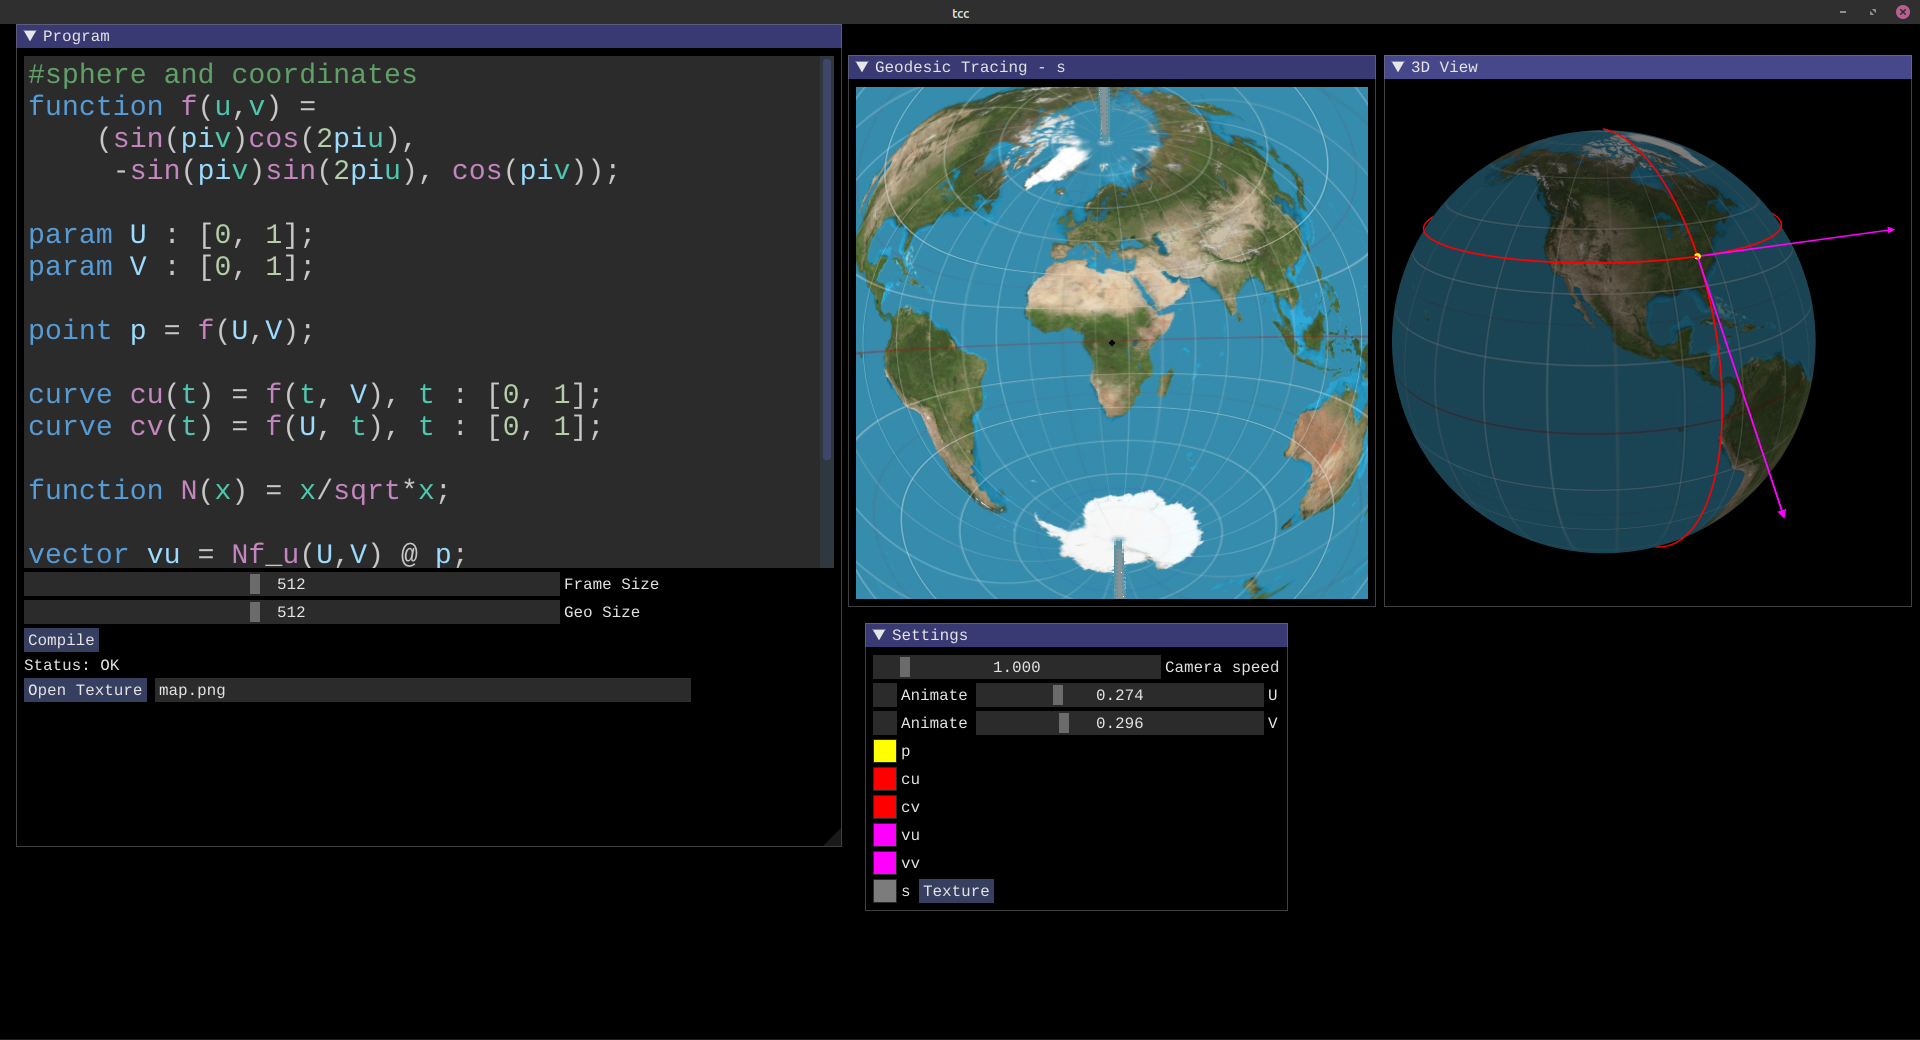
\includegraphics[width=\linewidth]{preview.png}
    \caption{Exemplo da visualização}
    \label{img:preview}
\end{figure}